\documentclass[10pt,twocolumn]{article}

\usepackage[margin=0.72in]{geometry}
\usepackage{amsmath,amssymb}
\usepackage{booktabs}
\usepackage{graphicx}
\usepackage{microtype}
\usepackage[numbers,sort&compress]{natbib}
\usepackage{placeins}
\usepackage{siunitx}
\usepackage[table]{xcolor}
\usepackage{tikz}
\usepackage{url}
\usepackage[hidelinks]{hyperref}
\usetikzlibrary{arrows.meta,positioning}

\newcommand{\QCA}{QCA}
\newcommand{\vect}[1]{\mathbf{#1}}
\setlength{\columnsep}{0.22in}

\title{Compact Quantum Channel Attention for Static ASL Recognition:\\
A Controlled Study with Parameter-Matched Baselines}
\author{}
\date{}

\begin{document}
\maketitle

\begin{abstract}
Hybrid quantum--classical vision models are easy to misread. A change in
accuracy can come from a pretrained backbone, from an added projection, or
from the parameter budget. The proposed method in this study is quantum
channel attention (\QCA{}). Pooled DenseNet121 features pass through an
eight-qubit variational bottleneck and return as channel gates. The block
contains 17,464 attention parameters. Squeeze-and-excitation (SE) at the same
site contains 131,072, a factor of $7.51$, and a classical MLP with the same
projection widths contains 17,480. With the backbone frozen, SE records the
highest three-seed mean accuracy at 1\%, 5\%, and 10\% of the Kaggle ASL
Alphabet training split. At 10\% the means are 91.12\% (SE), 90.93\% (MLP),
90.36\% (\QCA{}), and 90.19\% (no attention). The primary external test
unfreezes every DenseNet layer and holds out each of five MU HandImages
signers on 1,815 A--Z images. Equal-signer accuracy is 94.78\% without
attention, 94.55\% for the MLP, 94.50\% for proposed \QCA{}, and 93.72\% for
SE. Proposed \QCA{} reaches the highest pooled accuracy, 94.99\%, yet paired
signer-level tests do not separate it from the controls. The measurements
establish a compact proposed gate. A predictive quantum advantage is not
among the results.
\end{abstract}

\section{Introduction}
\label{sec:intro}

Static ASL alphabet recognition assigns one class label to a single hand
image. Convolutional networks already handle that problem when the test
photographs resemble the training photographs
\citep{wadhawan_2020_static,rastgoo_2021_survey}. A high score on a random
image split is a weak promise about a new person. Hand shape, camera, and
pose move with the signer, and continuous sign translation raises a further
linguistic problem that isolated alphabet frames do not contain
\citep{erdogan_2024_signer,camgoz_2018_slt}.

A variational circuit adds a second ambiguity. A classical optimizer can
train the circuit after a pretrained network has compressed the image
\citep{cerezo_2021_vqa,mari_2020_transfer,benedetti_2019_pqc}. If the hybrid
model then scores well, the credit might belong to the pretrained features,
to the extra projection, to a larger parameter budget, or to the circuit.
Classical simulations of quantum models are sensitive to exactly that choice
of baseline \citep{bowles_2024_benchmark,raubitzek_2023_applicability}.

Three shortcuts show up often enough to plan for them in advance. An easy
split can sit near the ceiling for every head, so the attention block never
gets a chance to matter. A quantum block can look helpful only because it
contains more parameters than the classical head it replaces. A pooled score
can follow the signer who contributed the most images. Figure~\ref{fig:evaluation-logic}
pairs each shortcut with the control used later: a low-data cut of the
training split, a parameter-matched MLP beside the larger SE block, and an
equal-signer average.

\begin{figure*}[t]
\centering
\resizebox{0.82\textwidth}{!}{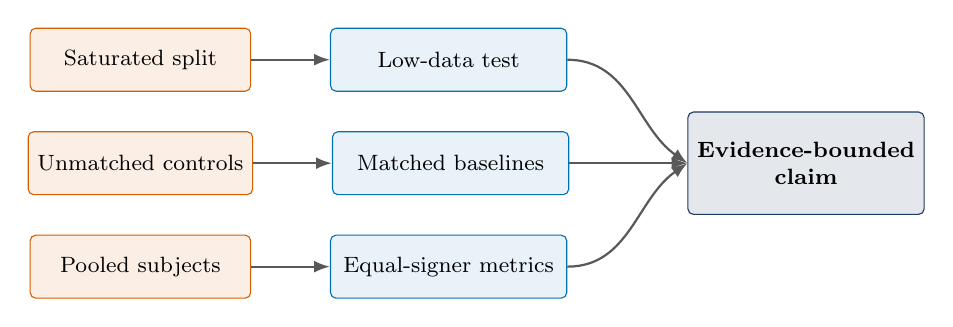
\begin{tikzpicture}[
  node distance=5mm and 10mm,
  risk/.style={draw=D55E00, fill=D55E00!10, rounded corners=2pt,
               minimum width=28mm, minimum height=8mm, align=center,
               font=\footnotesize},
  fix/.style={draw=0072B2, fill=0072B2!9, rounded corners=2pt,
              minimum width=30mm, minimum height=8mm, align=center,
              font=\footnotesize},
  claim/.style={draw=1F3A5F, fill=1F3A5F!12, rounded corners=2pt,
                minimum width=30mm, minimum height=13mm, align=center,
                font=\footnotesize\bfseries},
  flow/.style={-{Latex[length=2mm]}, thick, draw=gray!70!black}
]
\definecolor{D55E00}{HTML}{D55E00}
\definecolor{0072B2}{HTML}{0072B2}
\definecolor{1F3A5F}{HTML}{1F3A5F}

\node[risk] (sat) {Saturated split};
\node[risk, below=of sat] (unmatched) {Unmatched controls};
\node[risk, below=of unmatched] (pooled) {Pooled subjects};

\node[fix, right=of sat] (low) {Low-data test};
\node[fix, right=of unmatched] (matched) {Matched baselines};
\node[fix, right=of pooled] (balanced) {Equal-signer metrics};

\node[claim, right=15mm of matched] (claim) {Evidence-bounded\\claim};

\draw[flow] (sat) -- (low);
\draw[flow] (unmatched) -- (matched);
\draw[flow] (pooled) -- (balanced);
\draw[flow] (low.east) to[out=0,in=145] (claim.west);
\draw[flow] (matched) -- (claim);
\draw[flow] (balanced.east) to[out=0,in=-145] (claim.west);
\end{tikzpicture}
}
\caption{Three attribution risks and the control paired with each risk.}
\label{fig:evaluation-logic}
\end{figure*}

The proposed method is \QCA{}, an eight-qubit channel gate on DenseNet121
\citep{huang_2017_densenet}. The module compresses 1,024 pooled channels to
eight bounded rotation angles, mixes those qubits with two entangling layers,
and expands eight Pauli-$Z$ measurements into sigmoid channel weights. SE
remains in the study as a higher-capacity classical gate
\citep{hu_2018_se}, not as the proposed model. The matched MLP copies the
\QCA{} projection sizes and drops the circuit. A head with no attention is
the third control.

The study contributes three things, and the results section is where they
are checked.
\begin{itemize}
  \item A reproducible eight-qubit channel gate with 17,464 attention
  parameters and an explicit hand-off between the circuit simulator and the
  tensor device.
  \item A four-way comparison, at one insertion point, against no attention,
  SE, and a 17,480-parameter MLP, under shared data and a shared optimizer.
  \item A three-seed low-data ablation and a five-fold, fully unfrozen
  signer-held-out test. Together they show that the parameter reduction is
  real and that a reliable accuracy gain over the controls is not.
\end{itemize}

\section{Related Work}
\label{sec:related}

Variational algorithms train a parameterized circuit with a classical
optimizer. Accuracy, trainability, and efficiency are still open for that
family \citep{cerezo_2021_vqa,benedetti_2019_pqc}. Random circuits in
particular can lose gradient signal as the qubit count grows
\citep{mcclean_2018_barren}. Mitarai et al.\ showed that a shallow circuit
can still be fitted by tuning its parameters against expectation values
\citep{mitarai_2018_qcl}. Mari et al.\ carry the same idea into images: a
pretrained classical network extracts features, and a terminal circuit
produces the class decision \citep{mari_2020_transfer}. \QCA{} keeps the
pretrained extractor. The circuit does a different job. Eight measurements
become channel gates, and the class decision stays with a linear head.
Writing classical inputs into circuit angles is the feature-map step
discussed by Schuld and Killoran and, for kernel classifiers, by
Havl\'{i}\v{c}ek et al.\ \citep{schuld_2019_feature,havlicek_2019_feature}.
Those papers motivate the encoding. They do not forecast an ASL gain.

Other quantum vision designs answer different questions. Henderson et al.\
apply small circuits to local image patches and then continue with a
classical network \citep{henderson_2020_quanvolutional}. Cong et al.\ define
a quantum convolution for many-body quantum states, using a logarithmic
number of variational parameters in the number of qubits
\citep{cong_2019_qcnn}. Budiutama et al.\ place channel attention inside a
quantum convolutional network and evaluate quantum phase recognition
\citep{budiutama_2024_channel}. None of those settings is a gate on pooled
RGB features from a classical backbone, so their reported gains do not
transfer as numbers. Data re-uploading repeats the input encoding between
trainable blocks and can enlarge the set of functions a quantum classifier
represents \citep{perez_2020_reupload}. One fixed-budget re-uploading variant
appears later as a pilot. Greater expressivity is not treated as evidence
that the ASL head will improve.

On the classical side, SE recalibrates channels with a bottleneck MLP on
pooled features \citep{hu_2018_se}. That block is the high-capacity control.
A second control keeps the \QCA{} projection widths and removes the circuit,
which is the comparison that quantum-versus-classical benchmarks are prone
to skip \citep{bowles_2024_benchmark,raubitzek_2023_applicability}. Deep
models already recognize isolated static signs
\citep{wadhawan_2020_static}. Recent surveys cover a wide range of
hand-shape and motion pipelines \citep{rastgoo_2021_survey}. Signer identity
is a separate failure mode and needs an explicit held-out person
\citep{erdogan_2024_signer}. Video-to-text sign translation
\citep{camgoz_2018_slt} lies outside the static alphabet task studied here.

\section{Proposed Method}
\label{sec:method}

DenseNet121 \citep{huang_2017_densenet}, initialized from ImageNet
\citep{deng_2009_imagenet}, maps each input image to a pooled vector
$\vect{x}\in\mathbb{R}^{1024}$. An attention module returns
$\vect{a}\in(0,1)^{1024}$. The classifier receives
$\vect{x}'=\vect{x}\odot\vect{a}$. Proposed \QCA{} is the module that
builds $\vect{a}$. The no-attention control passes $\vect{x}$ straight to
the same classifier.

The gate has a short path. A linear map reduces 1,024 channels to eight
angles. Two entangling layers mix the eight qubits. Pauli-$Z$ measurements
return eight numbers, and a second linear map expands them into 1,024
sigmoid gates. The pooled features skip around the circuit and are only
rescaled, which keeps the backbone representation available to the
classifier. Figure~\ref{fig:qca-overview} draws that path. Classical stages
are marked separately from the circuit.

\begin{figure*}[t]
\centering
\resizebox{0.98\textwidth}{!}{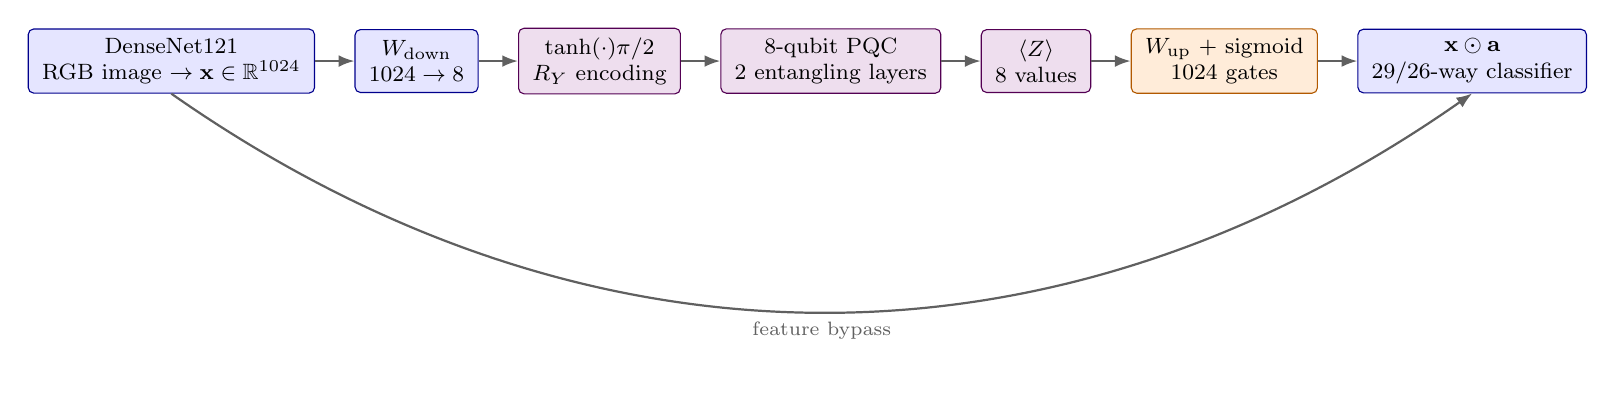
\begin{tikzpicture}[
  node distance=5mm,
  box/.style={draw, rounded corners=2pt, align=center, minimum height=8mm,
              inner xsep=5pt, font=\footnotesize},
  classical/.style={box, fill=blue!10, draw=blue!55!black},
  quantum/.style={box, fill=violet!13, draw=violet!65!black},
  gate/.style={box, fill=orange!15, draw=orange!70!black},
  flow/.style={-{Latex[length=2mm]}, thick, draw=gray!75!black}
]
\node[classical] (cnn) {DenseNet121\\RGB image $\rightarrow \mathbf{x}\in\mathbb{R}^{1024}$};
\node[classical, right=of cnn] (down) {$W_{\mathrm{down}}$\\$1024\rightarrow8$};
\node[quantum, right=of down] (encode) {$\tanh(\cdot)\pi/2$\\$R_Y$ encoding};
\node[quantum, right=of encode] (pqc) {8-qubit PQC\\2 entangling layers};
\node[quantum, right=of pqc] (measure) {$\langle Z\rangle$\\8 values};
\node[gate, right=of measure] (up) {$W_{\mathrm{up}}$ + sigmoid\\1024 gates};
\node[classical, right=of up] (classify) {$\mathbf{x}\odot\mathbf{a}$\\29/26-way classifier};

\draw[flow] (cnn) -- (down);
\draw[flow] (down) -- (encode);
\draw[flow] (encode) -- (pqc);
\draw[flow] (pqc) -- (measure);
\draw[flow] (measure) -- (up);
\draw[flow] (up) -- (classify);
\draw[flow] (cnn.south) to[out=-35,in=-145]
  node[below, font=\scriptsize, text=gray!75!black]{feature bypass} (classify.south);
\end{tikzpicture}
}
\caption{Proposed QCA gate on pooled DenseNet121 features.}
\label{fig:qca-overview}
\end{figure*}

The down-projection is bounded before it enters the circuit,
\begin{equation}
  \vect{z} = \tanh(W_d\vect{x}+\vect{b}_d)\frac{\pi}{2},
\end{equation}
so each coordinate lies in $(-\pi/2,\pi/2)$. That bounded encoding is the
concrete feature map used here \citep{schuld_2019_feature}. Eight $R_Y$
rotations load $\vect{z}$. Two layers of strongly entangling gates then mix
the register. The simulator returns
\begin{equation}
  q_i = \langle \psi(\vect{z},\vect{\theta})|Z_i|
  \psi(\vect{z},\vect{\theta})\rangle,\quad i=1,\ldots,8,
\end{equation}
and the up-projection is $\vect{a}=\sigma(W_u\vect{q}+\vect{b}_u)$. The
circuit is executed with PennyLane's \texttt{default.qubit} simulator, whose
gradients are available to a classical optimizer
\citep{bergholm_2018_pennylane,mitarai_2018_qcl}. The call runs on CPU. The
eight measurements move back to the accelerator for the up-projection. That
hand-off is required by the software stack. It is not a timing result, and
it is not evidence of a hardware advantage.

The four heads share $\vect{x}$ and share the linear classifier. Only the
channel map changes. No attention is the identity. The matched MLP keeps the
$1024\rightarrow8$ and $8\rightarrow1024$ maps, replaces the circuit with a
bias-free $8\rightarrow8$ layer, and applies $\tanh$ on both sides of that
layer. SE uses reduction 16, a ReLU bottleneck, and sigmoid gates
\citep{hu_2018_se}. \QCA{} is the proposed map.
Figure~\ref{fig:controls} isolates that single difference. The matched MLP
has 17,480 attention parameters, sixteen more than \QCA{}. SE has 131,072.
The counts are tabulated with the results, where they are part of the claim
being tested.

\begin{figure*}[t]
\centering
\resizebox{0.82\textwidth}{!}{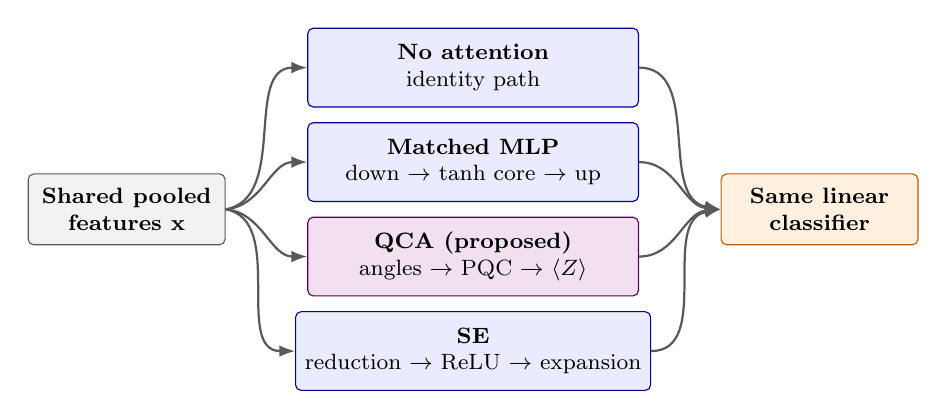
\begin{tikzpicture}[
  shared/.style={draw=gray!70!black, fill=gray!10, rounded corners=2pt,
                 minimum width=25mm, minimum height=9mm, align=center,
                 font=\footnotesize\bfseries},
  control/.style={draw=blue!60!black, fill=blue!8, rounded corners=2pt,
                  minimum width=42mm, minimum height=10mm, align=center,
                  font=\footnotesize},
  quantum/.style={draw=violet!70!black, fill=violet!12, rounded corners=2pt,
                  minimum width=42mm, minimum height=10mm, align=center,
                  font=\footnotesize},
  output/.style={draw=orange!75!black, fill=orange!12, rounded corners=2pt,
                 minimum width=25mm, minimum height=9mm, align=center,
                 font=\footnotesize\bfseries},
  flow/.style={-{Latex[length=2mm]}, thick, draw=gray!70!black}
]
\node[shared] (features) at (0,0) {Shared pooled\\features $\vect{x}$};

\node[control] (none) at (4.4,1.8) {\textbf{No attention}\\identity path};
\node[control] (mlp) at (4.4,0.6) {\textbf{Matched MLP}\\down $\rightarrow$ tanh core $\rightarrow$ up};
\node[quantum] (qca) at (4.4,-0.6) {\textbf{QCA (proposed)}\\angles $\rightarrow$ PQC $\rightarrow$ $\langle Z\rangle$};
\node[control] (se) at (4.4,-1.8) {\textbf{SE}\\reduction $\rightarrow$ ReLU $\rightarrow$ expansion};

\node[output] (head) at (8.8,0) {Same linear\\classifier};

\draw[flow] (features.east) to[out=10,in=180] (none.west);
\draw[flow] (features.east) to[out=5,in=180] (mlp.west);
\draw[flow] (features.east) to[out=-5,in=180] (qca.west);
\draw[flow] (features.east) to[out=-10,in=180] (se.west);

\draw[flow] (none.east) to[out=0,in=170] (head.west);
\draw[flow] (mlp.east) to[out=0,in=175] (head.west);
\draw[flow] (qca.east) to[out=0,in=-175] (head.west);
\draw[flow] (se.east) to[out=0,in=-170] (head.west);
\end{tikzpicture}
}
\caption{Shared features and classifier. QCA is the proposed channel map.}
\label{fig:controls}
\end{figure*}

\section{Experimental Protocol}
\label{sec:protocol}

Two protocols answer two questions. The frozen Kaggle runs ask whether the
head helps when the backbone cannot adapt. The MU runs train every DenseNet
layer and ask whether the full model holds up on a signer who was absent
from training. The same optimizer and epoch budget are used for every
method, so a gap is harder to dismiss as a tuning accident
\citep{raubitzek_2023_applicability,bowles_2024_benchmark}.

\subsection{Kaggle ASL Alphabet}

The collection contains 87,000 images and 29 labels: A--Z, \emph{del},
\emph{nothing}, and \emph{space}.\footnote{%
\url{https://www.kaggle.com/datasets/grassknoted/asl-alphabet}}
A stratified 80/10/10 split with seed 42 fixes 8,700 validation images and
8,700 test images. The official 28-image Kaggle test folder is unused. For
the controlled study the ImageNet-initialized extractor stays frozen, and
only the training partition is stratified down to 1\%, 5\%, or 10\%.
Validation and test stay intact. Each method trains for 15 epochs at seeds
42, 43, and 44, on $224\times224$ inputs, with batch size 32. The optimizer
is AdamW \citep{loshchilov_2019_adamw}, initial learning rate $0.001$,
weight decay $0.0001$, and a cosine schedule across the epoch budget
\citep{loshchilov_2017_sgdr}. The checkpoint with the best validation
accuracy is evaluated once on the held-out test set. Horizontal flips are
omitted because they change the handedness of a sign.

The frozen protocol is an attribution ablation. It does not describe a
deployment setting. Separate end-to-end checks on the full training split
reach 100\% test accuracy both for plain DenseNet121 and for DenseNet121
with \QCA{}. That tie is treated as evidence that the random image split is
saturated for comparing attention heads.

\subsection{MU Signer-Held-Out Study}

MU HandImages contains 2,425 frames from five people.\footnote{%
\url{https://hdl.handle.net/10179/4514}}
The study keeps 1,815 A--Z examples and drops the remaining classes, leaving
a 26-way task. The five signers contribute 650, 645, 130, 130, and 260
images. Each fold holds out one signer for testing and takes a
class-stratified 15\% of the other four signers as validation.

Every DenseNet layer is trainable. Training lasts 15 epochs at seed 42, with
$224\times224$ inputs, batch size 32, backbone learning rate $0.00001$, head
learning rate $0.001$, weight decay $0.0001$, AdamW, and cosine annealing
\citep{loshchilov_2019_adamw,loshchilov_2017_sgdr}. Checkpoint selection
follows the same validation rule in every fold.

\subsection{Metrics}

Reported figures are test accuracy and macro-F1, recomputed from the saved
checkpoint. Kaggle summaries are the mean and sample standard deviation
across three training seeds. For MU, the primary summary gives each signer
equal weight: the mean and sample standard deviation of the five fold
scores. Pooled scores concatenate the folds and therefore weigh a signer by
image count. Exploratory two-sided paired $t$-tests compare proposed \QCA{}
with each control on the five signer accuracies. The three tests are
unadjusted. Five pairs have little power, so a failure to reject the null
at $\alpha=0.05$ is not an equivalence result.

\section{Results}
\label{sec:results}

\subsection{Compactness of Proposed QCA}

The proposed method is \QCA{}. SE is a larger classical control. Treating
the highest score in a table as the proposed method would invert the study,
and it would make the signer-held-out comparison look like a failed SE
paper. The claim that the results can actually support is narrower, and it
is numerical.

Table~\ref{tab:parameters} records the parameter side of that claim. Proposed
\QCA{} has 17,464 attention parameters. The matched MLP has 17,480. SE has
131,072, which is $7.51\times$ the \QCA{} attention budget. Frozen trainable
counts follow the same order: 47,189 for \QCA{}, 47,205 for the MLP, 160,797
for SE, and 29,725 with no attention. Once the backbone is unfrozen, the
extractor dominates the total, so an unfrozen parameter count is not
evidence that the gate itself is small. The attention column is the relevant
one.

\begin{table}[!hb]
\centering
\caption{Parameter counts of all channel modules.}
\label{tab:parameters}
\resizebox{\columnwidth}{!}{%
\begin{tabular}{lrrr}
\toprule
Module & Attention & Trainable (frozen) & Trainable (full) \\
\midrule
\textbf{QCA (proposed)} & \textbf{17,464} & 47,189 & 6,997,970 \\
Matched MLP & 17,480 & 47,205 & 6,997,986 \\
SE ($r=16$) & 131,072 & 160,797 & 7,111,578 \\
No attention & 0 & 29,725 & 6,980,506 \\
\bottomrule
\end{tabular}}
\end{table}


\subsection{Signer-Held-Out Evaluation}

The predictive test of proposed \QCA{} is the fully unfrozen MU protocol.
Table~\ref{tab:mu} gives equal-signer means beside pooled scores. Under the
primary, equal-signer summary, no attention reaches 94.78\%, the matched MLP
94.55\%, proposed \QCA{} 94.50\%, and SE 93.72\%. Signer-level macro-F1 puts
no attention first as well. Proposed \QCA{} does lead the pooled accuracy,
at 94.99\%, ahead of the MLP at 94.88\%, no attention at 94.82\%, and SE at
94.71\%. The fold sizes differ by a factor of five, so the pooled number
answers a different question: performance on this particular mixture of
images. It does not answer performance for a typical held-out signer.
Two-sided paired tests of \QCA{} against no attention, the MLP, and SE
return $p=0.543$, $p=0.943$, and $p=0.116$. None rejects the null at
$\alpha=0.05$. Five signers cannot carry an equivalence claim either. The
supported reading is that proposed \QCA{} stays with the controls while
using far fewer attention parameters than SE. A ranking that flips when the
average changes is a known risk in small quantum-model comparisons
\citep{bowles_2024_benchmark}.

\begin{table*}[t]
\centering
\caption{Signer-held-out results for proposed QCA and the controls (\%).}
\label{tab:mu}
\small
\begin{tabular}{lrrrr}
\toprule
Method & Signer accuracy & Signer macro-F1 & Pooled accuracy & Pooled macro-F1 \\
\midrule
\textbf{QCA (proposed)} & $94.50 \pm 4.95$ & $94.26 \pm 4.94$ & $94.99$ & $94.97$ \\
Matched MLP & $94.55 \pm 4.02$ & $93.95 \pm 4.45$ & $94.88$ & $94.82$ \\
SE & $93.72 \pm 5.17$ & $93.04 \pm 5.43$ & $94.71$ & $94.63$ \\
No attention & $94.78 \pm 5.17$ & $94.61 \pm 5.28$ & $94.82$ & $94.77$ \\
\bottomrule
\end{tabular}
\end{table*}


The fold plot makes the spread obvious. Methods move together inside a
signer, and signers do not. Signer 5, the 260-image fold, is the low point
for every head. The gap between heads inside one fold is smaller than the
gap between signer 5 and the other four.
Figure~\ref{fig:signer} shows that pattern.

\begin{figure*}[t]
\centering
\includegraphics[width=0.90\textwidth]{../runs/mu_loso_signer_accuracy.png}
\caption{MU test accuracy of proposed QCA and the controls, by held-out signer.}
\label{fig:signer}
\end{figure*}

Table~\ref{tab:signers} lists the same folds. Proposed \QCA{} matches no
attention on signer 1 (95.38\%) and on signer 5 (85.77\%), and matches SE on
signer 2 (97.52\%). Signer 3 is the clearest local loss for \QCA{} relative
to no attention, 96.92\% against 98.46\%. No row wins every signer. That is
why the paired tests stay inconclusive, and why a single pooled percentage
would overstate the case for any one head \citep{erdogan_2024_signer}.

\begin{table*}[t]
\centering
\caption{Held-out signer accuracy for proposed QCA (\%; counts in parentheses).}
\label{tab:signers}
\small
\begin{tabular}{lrrrrr}
\toprule
Method & Signer 1 (650) & Signer 2 (645) & Signer 3 (130) & Signer 4 (130) & Signer 5 (260) \\
\midrule
\textbf{QCA (proposed)} & 95.38 & 97.52 & 96.92 & 96.92 & 85.77 \\
Matched MLP & 94.77 & 97.21 & 97.69 & 95.38 & 87.69 \\
SE & 95.69 & 97.52 & 95.38 & 95.38 & 84.62 \\
No attention & 95.38 & 96.59 & 98.46 & 97.69 & 85.77 \\
\bottomrule
\end{tabular}
\end{table*}


Errors of the proposed module, pooled over the five held-out signers, sit on
the diagonal except for a few letter pairs. The occupied off-diagonal cells
are led by M predicted as N, N predicted as M, and V predicted as W, with a
smaller A-to-T band. Those pairs are visually close in a still frame.
Figure~\ref{fig:qca-cm} prints the count in every occupied cell of that one
matrix, so the diagonal and the confusions can be read without a four-panel
reduction.

\begin{figure*}[t]
\centering
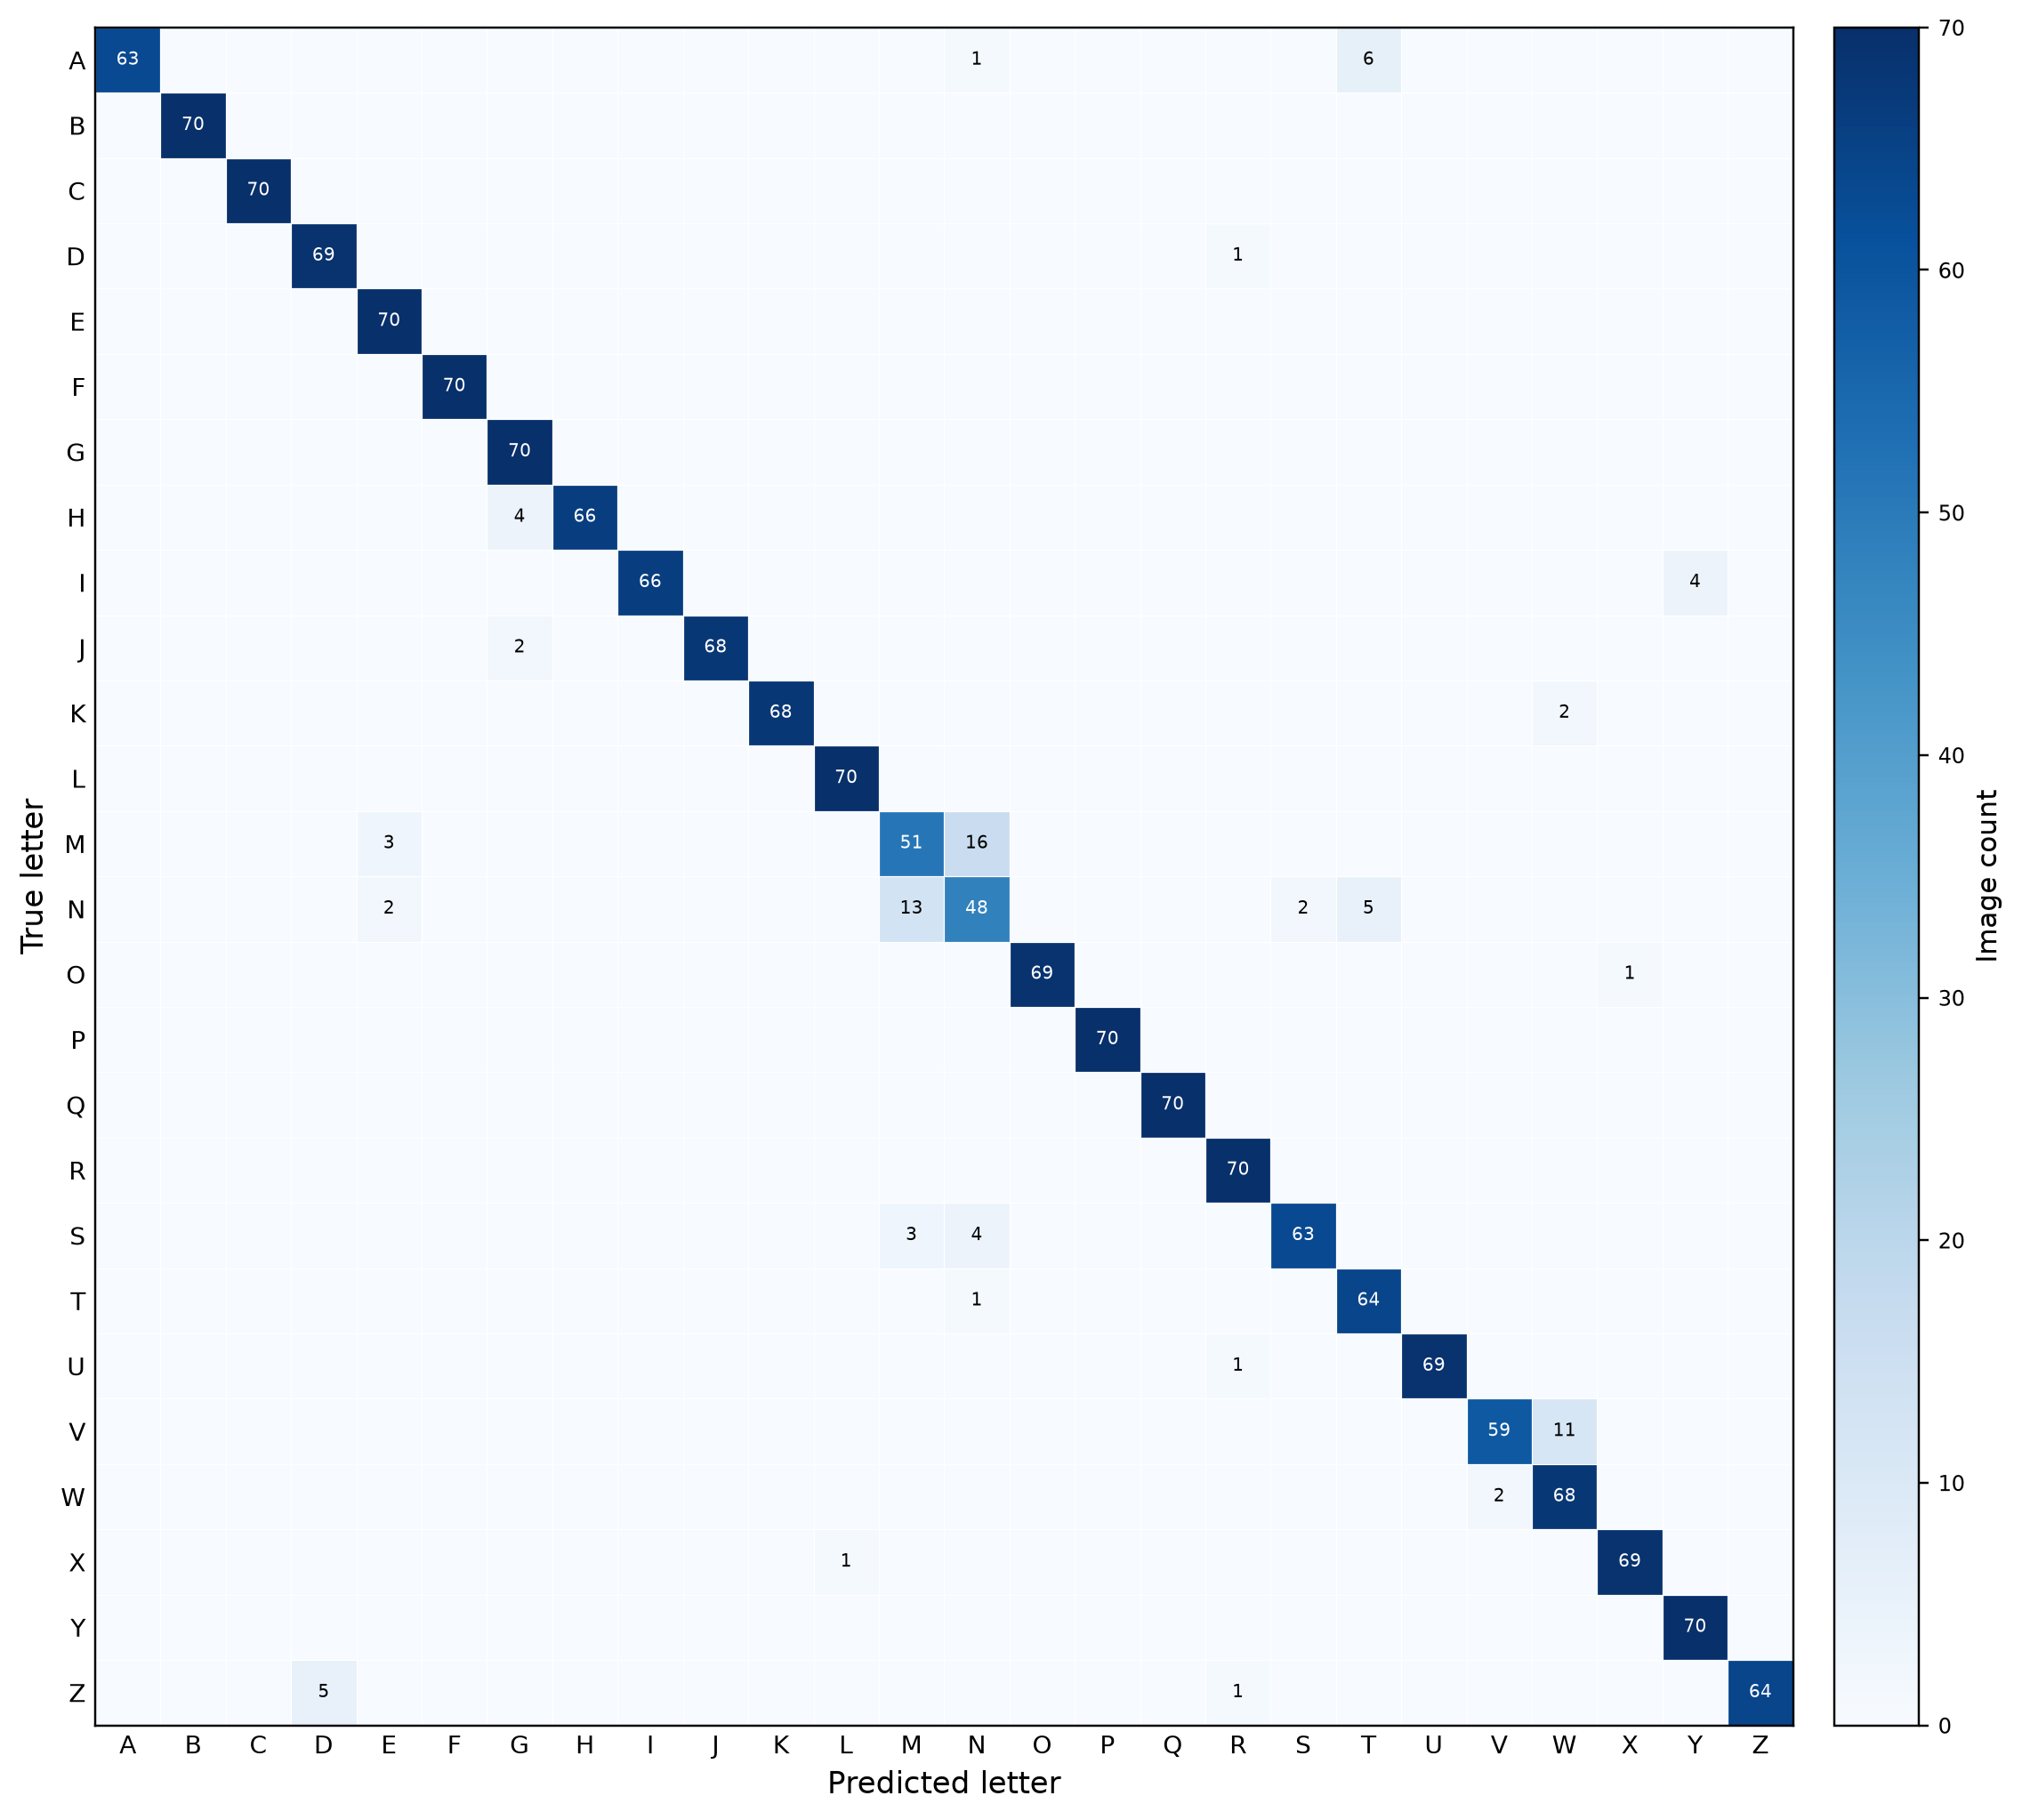
\includegraphics[width=0.92\textwidth]{figures/qca_confusion_matrix.png}
\caption{Pooled confusion matrix of proposed QCA on the five MU held-out signers.}
\label{fig:qca-cm}
\end{figure*}

\subsection{Frozen Low-Data Ablation}

The frozen runs ask a narrower question and do not change which method is
proposed. With the extractor fixed, extra capacity in the head is easier to
see. SE, the larger control of Hu et al.\ \citep{hu_2018_se}, has the
highest mean test accuracy at 1\%, 5\%, and 10\% of the training split.
Table~\ref{tab:low-data} reports the three-seed means. At 1\%, proposed
\QCA{} reaches 62.16\%, below SE at 66.17\% and below no attention at
64.69\%. At 5\%, \QCA{} is the lowest of the four means. At 10\%, the
matched MLP reaches 90.93\% and proposed \QCA{} reaches 90.36\%, just above
no attention at 90.19\%. The matched MLP is the informative control at that
fraction: nearly the same parameter count, higher accuracy.

\begin{table*}[t]
\centering
\caption{Frozen Kaggle test accuracy (\%; mean $\pm$ SD, three seeds).}
\label{tab:low-data}
\small
\begin{tabular}{lrrr}
\toprule
Method & 1\% training data & 5\% training data & 10\% training data \\
\midrule
\textbf{QCA (proposed)} & $62.16 \pm 1.16$ & $86.13 \pm 0.93$ & $90.36 \pm 0.35$ \\
Matched MLP & $60.80 \pm 1.31$ & $86.39 \pm 0.47$ & $90.93 \pm 0.24$ \\
SE & $66.17 \pm 0.42$ & $87.22 \pm 0.88$ & $91.12 \pm 0.45$ \\
No attention & $64.69 \pm 0.63$ & $86.43 \pm 0.55$ & $90.19 \pm 0.60$ \\
\bottomrule
\end{tabular}
\end{table*}


Figure~\ref{fig:low-data} plots those means with sample standard deviation.
All four curves rise and draw closer as the training fraction grows. SE
remains the upper curve at every marked fraction. The spread across seeds is
largest at 1\%, where \QCA{} and the MLP both move by more than a point
across the three initializations.

\begin{figure*}[t]
\centering
\includegraphics[width=0.86\textwidth]{../runs/low_data_learning_curve.png}
\caption{Frozen Kaggle test accuracy (mean $\pm$ SD over three seeds).}
\label{fig:low-data}
\end{figure*}

Macro-F1 preserves the accuracy order at each fraction.
Table~\ref{tab:low-data-f1} is the check that a single dominant class is not
hiding a different ranking. At 10\%, for example, proposed \QCA{} has macro-F1
90.35\% beside accuracy 90.36\%. The two metrics do not tell different
stories.

\begin{table*}[t]
\centering
\caption{Frozen Kaggle macro-F1 (\%; mean $\pm$ SD, three seeds).}
\label{tab:low-data-f1}
\small
\begin{tabular}{lrrr}
\toprule
Method & 1\% training data & 5\% training data & 10\% training data \\
\midrule
\textbf{QCA (proposed)} & $60.49 \pm 1.46$ & $86.06 \pm 0.94$ & $90.35 \pm 0.38$ \\
Matched MLP & $59.06 \pm 1.79$ & $86.34 \pm 0.50$ & $90.94 \pm 0.23$ \\
SE & $65.25 \pm 0.11$ & $87.18 \pm 0.90$ & $91.13 \pm 0.46$ \\
No attention & $63.42 \pm 0.92$ & $86.38 \pm 0.56$ & $90.17 \pm 0.62$ \\
\bottomrule
\end{tabular}
\end{table*}


A separate frozen run on the full training split, seed 42, agrees with the
low-data order. SE reaches 97.10\% test accuracy, proposed \QCA{} 95.98\%,
and no attention 95.89\%. SE's extra 1.12 points sit next to a
$7.51\times$ larger attention block. That is a real accuracy gap in the
frozen setting. It is also the reason SE cannot be quietly promoted to the
proposed method: the study set out to test whether the smaller quantum gate
was worth using, and the frozen answer is that the smaller gate gives up
accuracy.

\subsection{Data Re-uploading Pilot}

At 1\% training data and seed 42, a re-uploading variant that repeats the
eight-angle encoding before each variational layer reaches 61.38\% test
accuracy. The matched \QCA{} run without re-uploading reaches 61.83\%. Both
use 17,464 attention parameters. The variant does not improve the matched
seed, so the pilot stops there \citep{perez_2020_reupload}.

\section{Discussion}
\label{sec:discussion}

The result that survives both protocols is compactness, not a win on
accuracy. Proposed \QCA{} is the only new block in the comparison, and
Table~\ref{tab:parameters} fixes its size. SE is more accurate whenever the
backbone is frozen. The matched MLP, which is the control with almost the
same width, is at least as accurate as \QCA{} at 10\% training data and on
the equal-signer MU mean. A circuit effect that beat a same-sized classical
bottleneck would have shown up there. It does not.

The two protocols disagree because they ask different questions, which is
also why a benchmark can be tipped by its design
\citep{raubitzek_2023_applicability,bowles_2024_benchmark}. Freezing the
backbone isolates the head and, at the same time, refuses the extractor any
chance to adapt to ASL. End-to-end MU training is closer to a model one
might actually ship, and there the differences between heads are smaller
than the differences between signers. Signer identity has the same character
in other sign-recognition studies: a representation that fits the people in
the training set can fail on a new person \citep{erdogan_2024_signer}. The
full-data Kaggle split makes the attribution problem worse in another way.
Plain DenseNet121 and DenseNet121 with \QCA{} both reach the ceiling, so a
hybrid score of 100\% would have nothing to say about the circuit.

Subject weighting has to stay visible for the same reason. Pooled accuracy
describes the empirical mixture of images. The equal-signer mean describes
an average observed person. Proposed \QCA{} leads the first and does not
lead the second. Publishing only the pooled 94.99\% would invent a ranking
the signer-level tests do not support. Adding depth or qubits in the hope of
reversing that outcome is not a free next step. Gradient signal in random
parameterized circuits can collapse as the register grows
\citep{mcclean_2018_barren}. Any such sweep would also have to give the MLP
and SE the same tuning budget they were denied here.

\FloatBarrier
\section{Future Scope}
\label{sec:future}

The useful next measurement is a larger signer-held-out set: more people,
and more than one training seed. Five pairs cannot separate a
half-point gap from noise, and a single seed cannot show that the tie
survives a new initialization. Capture conditions and continuous signing
are still outside the static frames used here
\citep{camgoz_2018_slt,rastgoo_2021_survey}.

Hardware claims need a different experiment. Gate noise limits the circuit
that can be executed reliably, and a small device is not an automatic win
on a vision task \citep{preskill_2018_nisq}. A noise model, or a run on
hardware, has to come before any statement about speed, energy, or
robustness. Depth and qubit count belong in a preregistered sweep with the
same search budget on the classical controls, both because random circuits
can become untrainable \citep{mcclean_2018_barren} and because a
re-uploading construction \citep{perez_2020_reupload} already failed to help
at the one budget that was tried. The shared schedule in the present runs
keeps the methods comparable. It does not certify that each head was fully
tuned. The redistribution terms of the pinned MU mirror should also be
confirmed before derived images or predictions are released.

\FloatBarrier
\section{Conclusion}
\label{sec:conclusion}

The proposed method is an eight-qubit channel gate on pooled DenseNet121
features for static ASL recognition. The comparison that tests it uses no
attention, a parameter-matched MLP, and a much larger SE block, under one
data pipeline and one optimizer. Proposed \QCA{} meets the compactness
target: SE uses $7.51\times$ as many attention parameters. It does not meet
an accuracy target. SE leads every frozen low-data condition, and no
attention has the highest equal-signer mean once the backbone is trained.
The pooled edge for \QCA{} on MU disappears under equal-signer averaging
and is not supported by paired tests. What the study demonstrates is a
compact quantum channel gate whose predictive value, on these splits and
this simulator, stays inside the range of fair classical controls
\citep{bowles_2024_benchmark}.

\bibliographystyle{plainnat}
\bibliography{references}

\end{document}
